%-----------------------------------------------------------------------
% Cabecera del documento. Aqui se incluyen los paquetes y las
% definiciones que se utilizen despues en el documento.

\documentclass[a4paper,11pt]{article} % Tipo del documento. Puede ser
                                      % book, article, report, y
                                      % muchos mas

\usepackage{./estilos/estiloBase} % Basicamente son todas las
                                  % librerias usadas. En caso de que
                                  % falten librerias se van añadiendo
                                  % al fichero.
\usepackage{./estilos/colores}  % Algunos colores ya generados, para
                                % los algunos estilos más avanzados.
\usepackage{./estilos/comandos} % Algunos comandos personalizados

\title{GoM: Simulador de batallas fantásticas} % Título del documento
\author{Alumno: Aarón Bueno Villares\\Director: Manuel Palomo Duarte} % Autor (o
                                % autores)
\date{\today} % Fecha. La orden \today indica el dia de hoy con dia
              % mes y año. 

%----------------------------------------------------------------------

\begin{document} % Lo que este en el entorno document es lo que se va
                 % a mostrar finalmente.
\sinmargen
\maketitle % Generacion automatica del titulo o la portada si es un book.

\abstract{\noindent El siguiente documento se presenta a modo de resumen que
  complementa la memoria del mismo Proyecto Fin de Carrera, entregado el
  dia de la presentación de este proyecto. El proyecto que nos ocupa
  es la creación de un juego de guerra de táctica militar de corte
  fantástico-medieval, primer juego que sirve como alternativa digital
  y gratuita de los populares juegos de miniaturas de la misma corte.}

\tableofcontents % Genera automaticamente el indice. Es necesario
                 % compilar dos veces para que este salga.

\section{Introducción}

\noindent Los juegos de guerra fantásticos de táctica por turnos son muy
demandados dentro del ámbito de los juegos de mesa. Una prueba de
ello es la popularidad de la que goza la empresa \emph{Games
  Workshop}, una empresa que se dedica, entre otras muchas cosas, a
mantener dos juegos muy populares y famosos de táctica militar por
turnos, \emph{Warhammer Fantasy Battles}, de corte fantástico, y
\emph{Warhammer 40k}, de corte futurista.

\noindent Debido al éxito entre los jóvenes y adolescentes, cada vez
de corta edad, de estos juegos, la empresa tuvo que adaptarse a sus
nuevos clientes, y el juego, a gusto de otros públicos, se hizo algo infantil.\\

\noindent También los precios se incrementaron debido a que ahora, los
compradores son madres en vez de adolescentes, que tienen menor disponibilidad
económica. Este hecho sobre todo fue el incentivo de que gran cantidad
de jugadores mas adultos dejaran el hobby.\\

\noindent El siguiente paso obvio fue buscar una alternativa digital a
este paradigma de juego. Tal búsqueda resultó una quimera ya que no
existía tal alternativa en la oferta de videojuegos. Todos los juegos
por turnos que hay son juegos de guerra de corte moderno, es decir,
cuyo componente principal es la artillería y las formaciones abiertas
con mucha movilidad, y no del elegante paradigma de guerra clásico que
existía antes de la popularización de la polvora.\\

\noindent \emph{GoM} pretende ofrecer (por primera vez en la
historia, por cierto) una alternativa digital a este paradigma de
juego con tanta popularidad, con el incentivo de ser libre, para
incentivar su mas rápida expansión, además de ser gratuito.\\

\noindent \emph{GoM}, al igual que \emph{Warhammer Fantasy} y otros
tantos juegos de táctica (no digitales) que han existido en la
historia de los juegos de guerra, está basado en un reglamento que
especifica exáctamente como resolverá \emph{GoM} cada una de las
acciones, y en concreto, qué acciones son las permitidas.\\

\noindent Los juegos tácticos por turnos tienen el aliciente de tener
un mayor control y un conocimiento mas profundo sobre sus tropas, y,
además, como también cuentan con el factor suerte (muchas de las
decisiones se modelan mediante números aleatorios, como en el
resultado de los combates), añaden mas tensión al juego.

\section{Calendario}
\noindent
El desarrollo del sistema ha seguido modelo de desarrollo iterativo
incremental, donde a cada iteración se completaba e implementaba una
nueva faceta de la aplicación, hasta conseguir un reglamento
implementado completo, rígido y suficiente.\\

\noindent
En la figura \ref{fig:gantt} podemos ver las iteraciones y/o ciclos en
las que se ha divido el desarrollo del sistema:

\begin{itemize}
\item Definición inicial (\ref{sec:def})
\item Arquitectura general del sistema (\ref{sec:arq})
\item Fase de movimiento (\ref{sec:mov})
\item Fase de combate (\ref{sec:com})
\item Interfaz gráfica (\ref{sec:graf})
\item Fase de disparos y magia (\ref{sec:disp})
\item Memoria (\ref{sec:mem})
\end{itemize}

\begin{figure}[h]
  \centering
  \includegraphics[scale=.5]{./imagenes/Gantt.png}
  \caption{Diagrama de Gantt del calendario del proyecto}
  \label{fig:gantt}
\end{figure}

\section{Iteraciones de desarrollo}
\noindent
Se dedicará una sección para cada una de las iteraciones de desarrollo
del proyecto.

\subsection{Definición inicial}
\label{sec:def}
\noindent
Esta iteración contiene las reflexiones iniciales del proyecto, así
como la obtención de documentación sobre el contexto de \emph{GoM} en
la diversidad y oferta de videojuegos, la confección de un reglamento
inicial como punto de partida para el desarrollo consecuente y la toma
de requisitos generales del mismo: interfaz gráfica 2D, librerias,
propiedades del sistema, etc.

\subsection{Arquitectura general del sistema}
\label{sec:arq}
\noindent
Una vez confeccionado un reglamento, se generó una arquitectura
general del sistema que sirviera como punto de partida en su
implementación.\\

\noindent
Se identificó una capa de dominio llamado gestor de reglas, que
implementaría al reglamento y fuera su motor, y una capa de
presentación que fuera el gestor de interfaz, que se intercomunicaría
con el gestor de reglas para pedirle la información que debe mostrar
al usuario.\\

\noindent
El gestor de reglas dispone de una clase llamada estado que guarda el
estado actual de la partida. El usuario realiza sus acciones enviándo
sus ordenes al gestor de interfaz, éste, envía la petición al gestor
de reglas. Toda nueva acción provocará un cambio de estado en el
sistema; el gestor de reglas, por tanto, con la acción recibida
cambiará el estado interno del juego y lo devolverá al gestor de
interfaz para que éste lo imprima. El diagrama de clases se muestra en
la figura \ref{fig:arqgen}.

\begin{figure}[h]
\centering
\includegraphics[scale=.8]{./imagenes/DiagramaJuego.png}
\label{fig:arqgen}
\caption{Arquitectura general del sistema}
\end{figure}

\noindent
A su vez, el gestor de reglas se descompone en otros gestores mas
concretos que se encargan de las acciones específicas de las distintas
fases de un turno de juego, como muestra la figura \ref{fig:reglas}.

\begin{figure}[h]
\centering
\includegraphics[scale=.8]{./imagenes/Reglas.png}
\label{fig:reglas}
\caption{Gestor de reglas}
\end{figure}

\subsection{Fase de movimiento}
\label{sec:mov}
\noindent
Ésta es quizás la fase mas crucial de la capa de dominio. La fase de
movimiento, como clase del sistema, solo se encarga de organizar y
discriminar las acciones disponibles en cada momento dentro de la fase
de movimiento, y podemos decir que es una clase sencilla, pero el
diseño e implementación de esta clase trajo consigo el diseño e
implementación del gestor de escenarios, una clase auxiliar que se
encarga de todo el cálculo numérico del juego. Se llama gestor de
escenario porque todos estos cálculos vienen referidos a la relación
de una unidad con el resto de unidades dentro de una batalla.\\

\noindent
Por lo que este ciclo de desarrollo se reduce o es sinónima del
desarrollo de este gestor de escenario (\ref{fig:escenario}). El
gestor de interfaz también interactúa con esta clase ya que necesita
cierta información para ofrecer al usuario la forma de responder a sus
peticiones, por ejemplo, para que un usuario mueva una unidad,
necesita saber cual es su desplazamiento máximo. El gestor de interfaz
pide esta información al gestor de escenario, hace los cálculos
oportunos, y devuelve el dato. El gestor de interfaz a continuación
imprime en el escenario un área transparente que indica la zona
disponible de movimiento.

\begin{figure}[h]
\centering
\includegraphics[scale=.8]{./imagenes/Escenario.png}
\label{fig:escenario}
\caption{Gestor de escenario}
\end{figure}

\subsection{Fase de combate}
\label{sec:com}
\noindent
En esta iteración se analizó, diseñó e implementó ampliamente la fase
de combate y todas las acciones involucradas en él. Se hicieron
bastantes cambios en el reglamento y luego éstos fueron
implementados.\\

\noindent
Estructuralmente esta fase es sencilla, aunque posee muchos cálculos
discretos cuya mayor dificultad es el propio caos de información que
hace falta manejar para gestionar todos y cada uno de los combates
(flancos, unidades combatientes en cada combate, ataques sin asignar,
etc).

\subsection{Interfaz gráfica}
\label{sec:graf}
\noindent
Antes de esta iteración, lo que se tenía en la capa de presentación
era sencillamente una interfaz gráfica sencilla que solo servía para
mostrar las unidades y poder hacer pruebas y ver los resultados de las
implementaciones anteriores.\\

\noindent
En esta iteración por fin se resolvió implementar la interfaz
diseñada, es decir, el menú y una presentación de la batalla mas
estéticos y completo, implementando también al gestor de ejércitos,
que permite manejar una serie de ejércitos, que pueden ser creados y
modificados por los usuarios, que quedarán grabados en el sistema y
podrán ser usados en las partidas.\\

\noindent
El gestor de interfaz se diseñó considerando a un gestor de iconos
como entidad separada del resto, que se encargaba de mostrar todos los
iconos del juego según las acciones disponibles en cada momento de la
batalla, imprimiéndolos en el orden y posición adecuada.\\

\noindent
A su vez, se usó un gestor de textos (cuya clase se llamó ListaTexto),
se permitía manejar de forma abstracta una lista de items textuales a
los que poder, de forma sencilla y cómoda, acceder, eliminar,
modificar, marcar, etc.\\

\noindent
En la figura \ref{fig:interfaz} se muestra el diagrama de clases usado
para implementar toda la funcionalidad ofrecida por el gestor de interfaz.

\begin{figure}[h]
\centering
\includegraphics[scale=.8]{./imagenes/Interfaz.png}
\label{fig:interfaz}
\caption{Gestor de intefaz}
\end{figure}

\subsection{Fases de disparo y magia}
\label{sec:disp}
\noindent
En esta iteración se incluyó en el sistema el gestor de disparo
mostrado en la figura \ref{fig:arqgen} y el sistema de magia que, por
su sencillez y simplicidad, se añadió los correspondientes cálculos de
control en los puntos adecuados de los otros gestores.

\subsection{Memoria}
\label{sec:mem}
\noindent
En esta última iteración se realizó la memoria del proyecto.

\section{Principales problemas de implementación}
\noindent
Se mostrará algunos de los problemas de implementación numéricos a los
que tuve que enfrentarme en la confección del gestor de escenarios.

\subsection{Desplazamiento máximo}
\noindent
El problema del desplazamiento máximo es el hecho de saber qué
distancia máxima tiene disponible una unidad para desplazarse al
frente. Esta capacidad tiene como cota máxima el valor del atributo de
movimiento base de la unidad, y se va reduciendo a medida que se
encuentran mas unidades por el camino.\\

\begin{minipage}[h]{0.4\columnwidth}
\centering
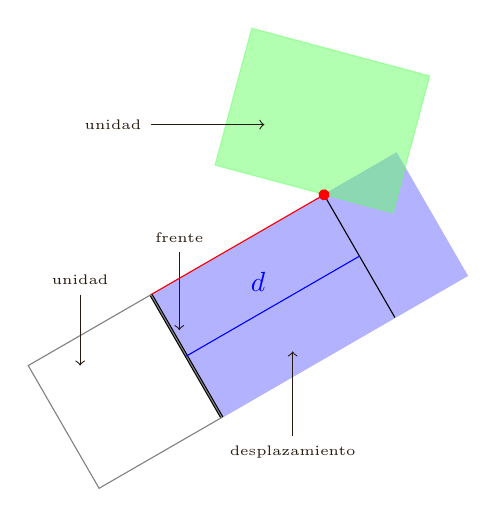
\begin{tikzpicture}[scale=1.8]
\filldraw[rotate=300,blue!30] (0,0) -- (1,0) -- (1,2) -- (0,2) --
cycle;
\filldraw[rotate=300,very thick] (0,0) -- (1,0);
\draw[brown!20!black,->] (.2,.3) node[above] {\tiny{frente}} -- (0.2,-.25);
\filldraw[rotate=345,opacity=.5, green!60] (0.2,1) -- (1.5,1) -- (1.5,2) -- (0.2,2) -- cycle;
\draw[rotate=300,gray,thin] (0,0) -- (1,0) -- (1,-1) -- (0,-1) --
cycle;
\draw[rotate=30,red] (0,0) -- (1.41,0);
\draw[rotate=30,black] (1.41,0)  -- (1.41,-1);
\draw[rotate=30,blue] (0,-0.5) -- (1.41,-0.5);
\draw[rotate=30,blue] (0.7,-0.3) node {$d$};
\filldraw[red,rotate=30] (1.41,0) circle(1pt);
\draw[brown!20!black,->] (-.5, 0) node[above] {\tiny{unidad}} -- (-.5, -.5);
\draw[brown!20!black,->] (1,-1) node[below] {\tiny{desplazamiento}}  --
(1,-.4);
\draw[brown!20!black,->] (0,1.2) node[left] {\tiny{unidad}} -- (.8,1.2);
\end{tikzpicture}
\end{minipage}
\begin{minipage}[h]{0.45\columnwidth}
La forma de resolver este problema, como ilustra la figura de la
izquierda, consiste en explorar todas las unidades presentes en el
campo de batalla y, para cada una de ellas, buscar todas las posibles
intersecciones (de aristas y vértices) con el rectángulo de movimiento
base, quedándonos con la distancia mínima de entre todas las distancias a
estos puntos de intersección.\\

\noindent
Para no violar la regla del espacio entre unidades incluida en el
reglamento, inicialmente se engrosa a la unidad esta misma cantidad, y
así este espacio de respeto queda incluido de forma intrínseca a la búsqueda.
\end{minipage}

\subsection{Pivotaje máximo}
\noindent
De forma análoga al problema anterior, este problema consiste en saber
cual es la capacidad de pivotaje máxima de una unidad, en relación al
resto de unidades presentes. Pivotar es el acto de que una unidad
cambie su encaración como resultado de mover la unidad mantiendo una
esquina de la formación como eje.\\

\noindent
Para resolver este cálculo, se toma una semicircunferencia cuyo arco
mide la capacidad de movimiento base de la unidad. Luego, para cada
unidad del campo de batalla, y al igual que en el caso anterior, se toman los
puntos de intersección con dicha semicircunferencia.\\

\begin{minipage}[h]{0.5\columnwidth}
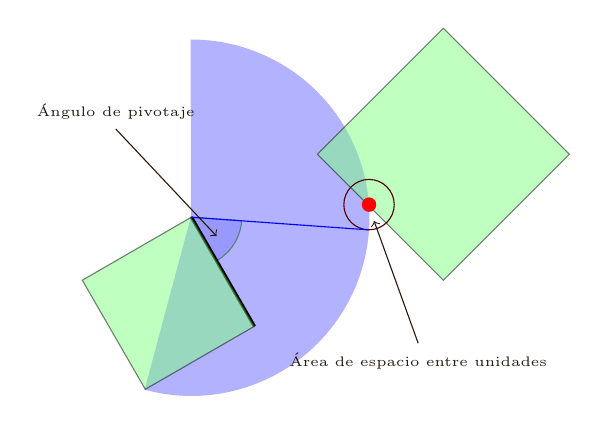
\begin{tikzpicture}[scale=1.6]
\filldraw[blue!30,rotate=300] (0,0) -- (1,-1) arc (-45:150:1.41cm) --
cycle;
\filldraw[opacity=.5,blue!50, draw=green!40!black,rotate=300] (.4,0) arc(0:56:.4cm) -- (0,0) -- cycle;
\draw[very thick, rotate=300] (0,0) -- (1,0);
\filldraw[opacity=.5,rotate=300,green!50,draw=black] (0,0) -- (1,0) --
(1,-1) -- (0,-1) -- cycle;
\filldraw[opacity=.5,green!50,draw=black] (1,.5) -- (2,1.5) --
(3,0.5) -- (2,-.5) -- cycle;
\filldraw[red] (1.41,.1) circle(1.5pt);
\draw[red!30!black] (1.41,.1) circle(.2cm);
\draw[blue] (0,0) -- (1.4,-.1);

\draw[brown!20!black,->] (1.8,-1) node[below] {\tiny{Área de espacio
    entre unidades}}-- (1.45,-.03);
\draw[brown!20!black,->] (-.6,.7) node[above] {\tiny{Ángulo de pivotaje}}-- (.2,-.15);
\end{tikzpicture}
\end{minipage}
\begin{minipage}[h]{0.34\columnwidth}
Como hemos de respetar la regla de la seperación de unidades, para
cada punto de intersección tomamos una circunferencia cuyo radio es dicho
espacio de separación. Como ilustra la figura, estos puntos obtenidos
tras buscar sus rectas tangentes desde el origen de la
semicircunferencia original serán los
tomados en consideración para ir acotando el ángulo de pivotaje máximo
de la unidad.
\end{minipage}

\subsection{Visión de una unidad}
\noindent
Caracterizar la visión de una unidad es establecer cuando una unidad
ve a otra. Esto depende de la cantidad de objetos que hayan en el
camino. A mayor cantidad de objetos, menor es la probabilidad de que
una unidad vea a la otra.\\

\noindent
Lo que se busca entonces es, para cada pareja de unidades, construir
el número máximo de rectángulos posibles, desplazados en cantidades
discretas, que se proyecten desde una unidad a la otra.

\noindent
\begin{minipage}[h]{0.4\columnwidth}
Para cada rectángulo, si existe al menos una unidad que tenga
intersección con dicho rectángulo o haz de visión, el rectángulo será
desechado. Si sobrevive al menos un rectángulo, podremos admitir que
la primera unidad ve a la segunda.\\

Dicho de otro modo, en cuanto
encontremos el primer rectángulo completamente limpio finalizamos la
búsqueda y admitimos que existe visibilidad entre las unidades.
\end{minipage}
\begin{minipage}[h]{0.5\columnwidth}
\centering
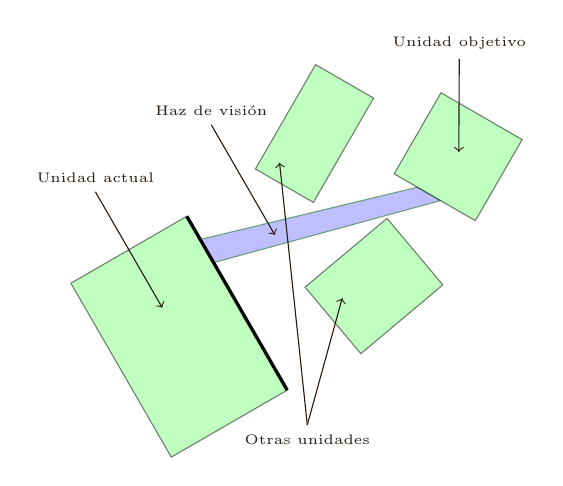
\begin{tikzpicture}[
  scale=1.7,
  rotate=300,
  unidad/.style={opacity=.5,green!50,draw=black},
  area/.style={opacity=.5,blue!50, draw=green!40!black},
  descripcion/.style={brown!20!black,->},
  ]
\coordinate (A) at (0,1);
\coordinate (B) at (1.5,1);
\coordinate (C) at (1.5,0);
\coordinate (D) at (0,0);

\coordinate (a) at (.5,2.5);
\coordinate (b) at (1.2,2.5);
\coordinate (c) at (1.2,3.2);
\coordinate (d) at (.5,3.2);

\coordinate (REF) at (a);
\coordinate (CENTRO) at (.75,1);

\filldraw[area] (0.4,1) -- (0.2,1) -- ({.5 + .2*cos(30)}, {2.5 + .2*sin(30)})--
+({.2*cos(30)}, {.2*sin(30)}) -- cycle;

\filldraw[unidad] (A) rectangle (C);

%No se por que no funciona girar coordenadas (c).
\filldraw[unidad,rotate around={30:(REF)}] (a) rectangle (1.2,3.2);

\coordinate (alfa) at (.9,1.5);
\coordinate (beta) at (1.4,2.4);

\filldraw[unidad,rotate around={10:(alfa)}] (alfa) rectangle (beta);

\filldraw[unidad,rotate around={30:(-.5,2.4)}] (0,1.5) rectangle
(-.5,2.4);

\draw[descripcion] (-.5,.5) node[above]{\tiny{Unidad actual}} --
(.5,.5);
\draw[descripcion] (-.5,1.5) node[above]{\tiny{Haz de visión}} --
(.45,1.5);

\coordinate (refunidades) at (1.8,1);

\draw[descripcion] (refunidades) node[below]{\tiny{Otras unidades}} --
(1.11,1.7);

\draw[descripcion] (refunidades) -- (0,1.8);

\draw[very thick] (A) -- (B);

\coordinate (refunidadobjetivo) at (0,3.35);

\draw[descripcion] (refunidadobjetivo) node[above]{\tiny{Unidad
    objetivo}} -- (.6,3);
\end{tikzpicture}
\end{minipage}

\subsection{Movimiento de huida}
Cuando una unidad huye, se genera un valor aleatorio entre la mitad y
el triple de la capacidad de movimiento de la unidad que va a huir.
Si la posición final de la unidad, según este nuevo valor, está
ocupado, la posición final de la unidad que huye será el siguiente
espacio libre encontrado.

\noindent
\begin{minipage}[h]{.35\columnwidth}
Para ello, en cada unidad presente en el camino, trazamos un par de
rectas discriminantes para cada unidad, una justo delante suya, que
llamaremos proximal, y otra justo detrás suya, que llamaremos recta
distal. Son las que hemos puesto de color rojo en la
figura.\\

Para cada unidad, obtenemos el espacio que existe entre la recta
distal de la primera unidad y la recta proximal de la siguiente.
Si este espacio es mayor a la profundidad de la unidad, significará que la 
unidad cabe en dicho espacio, y la primera posición encontrada que
cumpla con estas propiedades será la posición elegida final para
colocar a la unidad que está huyendo.
\end{minipage}
\begin{minipage}[h]{.5\columnwidth}
\centering
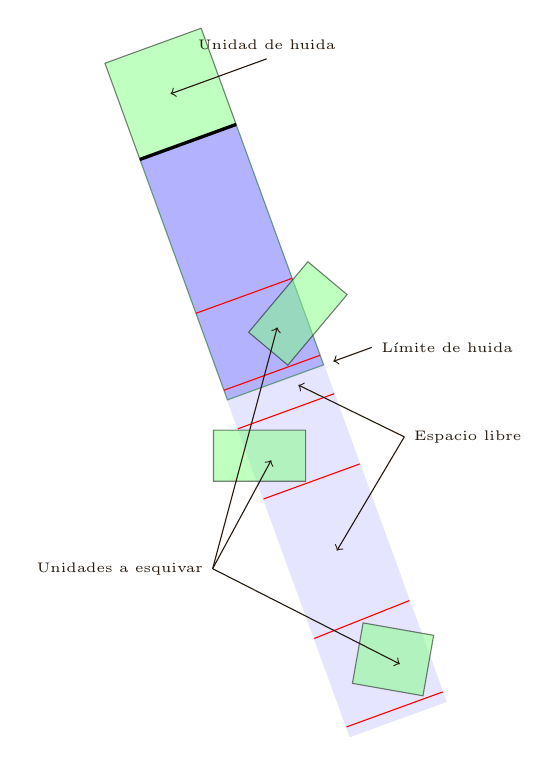
\begin{tikzpicture}[
  scale=1.3,
  rotate=200,
  unidad/.style={opacity=.5,green!50,draw=black},
  area/.style={opacity=.5,blue!50, draw=green!40!black},
  fondo/.style={blue!10},
  descripcion/.style={brown!20!black,->}
  ]

\filldraw[fondo] (0,1) rectangle (1,7);
\filldraw[area] (0,1) rectangle (1,3.5);
\filldraw[unidad] (0,0) rectangle (1,1);
\draw[very thick] (0,1) -- (1,1);
\filldraw[unidad, rotate around={30:(-.2,2.5)}] (-.2,2.5) rectangle
(.7,3);
\filldraw[unidad, rotate around={160:(1.4,4.2)}] (1.4,4.2) rectangle
(2.3,4.7);
\filldraw[unidad, rotate around={150:(.5,6)}] (.5,6) rectangle
(1.2,5.4);

\draw[red] (0,2.6) -- (1,2.6);
\draw[red] (0,3.4) -- (1,3.4);
\draw[red] (0,3.8) -- (1,3.8);
\draw[red] (0,4.53) -- (1,4.53);
\draw[red] (0,5.95) -- (1,5.98);
\draw[red] (0,6.9) -- (1,6.9);

\draw[descripcion] (-.5,.5) node[above]{\tiny{Unidad de huida}} --
(.5,.5);
\draw[descripcion] (-.5,4.43) node[right]{\tiny{Espacio libre}}
-- (.3,3.6);
\draw[descripcion] (-.5,4.43) -- (.5,5.25);
\draw[descripcion] (1.7,5) node[left]{\tiny{Unidades a esquivar}} --
(.3, 6.5);
\draw[descripcion] (1.7,5) -- (.8,4.2);
\draw[descripcion] (1.7,5) -- (.3,3);
\draw[descripcion] (-.5,3.5) node[right]{\tiny{Límite de huida}}--
(-.1,3.5);
\end{tikzpicture}
\end{minipage}

\section{Pruebas}
\noindent
Hemos distinguido dos fases de pruebas, las pruebas alfa, que son las
efectuadas durante el proceso de desarrollo, y las pruebas betas,
realizadas al finalizar este por mí y por otros compañeros.\\

\noindent
En las pruebas alfa, se pueden distinguir entre pruebas unitarias y
pruebas de integración. En las primeras, se diseñaban según criterios
de caja blanca y de cobertura de sentencias, esto es, probando la
implementación de las funciones vistas desde dentro, y procurando
explorar todas las ramas de ejecución posibles. Estas pruebas fueron
las usadas principalmente en la capa de dominio del juego. Por el
contrario, las pruebas de integración fueron las usadas en la capa de
presentación, pues es aquí donde cobra sentido el hecho de que todas
las clases y todo el juego en general actúe de forma conjunta
correctamente.\\

\noindent
En las pruebas beta se detectaron fallos solamente muy concretos y en
ocasiones muy excepcionales del juego, pues la mayoría de los errores
fueron satisfactoriamente encontrados con las pruebas unitarias.

\section{Conclusiones}
\noindent
En la realización del proyecto he aprendido lo importante que es el
buen orden y el uso de la metodología en la creación de software. La
creación del software es muy compleja y hacen falta ciertas
directrices generales, que por lo general son creadas desde la
experiencia de terceras personas. Aunque desde el comienzo hice un
análisis y diseño del software, en muchas ocasiones he hechado de
menos no haberme detenido aún mas tiempo en el estudio abstracto del
problema antes de ponerme directamente a implementar.

\nocite{pressman}
\nocite{laur04}
\nocite{raym01}
\nocite{stal04}
\nocite{mitt04}
\nocite{sdlweb}
\nocite{sdlosluca}
\nocite{cppref}
\nocite{warh}

\clearpage
\phantomsection
\addcontentsline{toc}{section}{Bibliografía y referencias}
\bibliographystyle{plain}
\bibliography{bibliografia.bib}

\end{document}
